\section{Interagujúce elektróny v čistom kove: Hartreeho - Fockova aproximácia pre model želé}
\label{sec:free_electrons}

Kvantová mechanika popisuje stav častice vlnovou funkciou $\Psi(\vec r,t)$, pomocou ktorej
je daná hustota pravdepodobnosti výskytu častice
\begin{equation}
\label{eq:fp2}
 \rho(\vec r, t)=\Psi(\vec r, t)\Psi^\ast(\vec r, t)\text{.}
\end{equation}
Keď sa častica nachádza v objeme $V$, hustota pravdepodobnosti je normalizovaná ako
\begin{equation}
\label{eq:norm}
 \int_{V} d \vec r  \  \rho(\vec r,t) = 1 \ .
\end{equation}
Vlnová funkcia voľnej častice je DeBroglieho rovinná vlna
\begin{equation}
\label{eq:fp}
 \Psi(\vec r,t)=Ce^{i(\vec k\cdot\vec r-\frac{E(k)t}{\hbar})} \text{,}
\end{equation}
kde $C$ je konštanta, $\hbar \vec k$ je hybnosť častice, a
\begin{equation}
 \label{eq:fp_erg}
 E(k)=\frac{\hbar^2 k^2}{2 m} \text{}
\end{equation}
je energia častice. Rovinná vlna sa dá normalizovať na konečný objem $V = L_xL_yL_z$,
ak uvažujeme priestor rozdelený na kvádre so stranami $L_x$, $L_y$ a $L_z$ a predpokladáme 
periodické Born vonKarmanove okrajové podmienky
\begin{equation}
 \Psi(x,y,z)=\Psi(x+L_x,y,z)\\, \\\ \Psi(x,y,z)=\Psi(x,y+L_y,z)\\, \\\ \Psi(x,y,z)=\Psi(x,y,z+L_z) \text{.}
\end{equation}
Pre rovinnú vlnu normovanú na kváder $V = L_xL_yL_z$ nam normovacia podmienka \eqref{eq:norm}
\begin{equation}
\label{eq:norm_bvk}
 \int_{0}^{L_x}  \int_{0}^{L_y}  \int_{0}^{L_z} dx dy dz  CC^\ast = 1\text{,}
\end{equation}
z ktorej vypočítame normovaciu konštantu
\begin{equation}
 \label{eq:A}
 C=\sqrt{\frac{1}{L_xL_yL_z}} = \sqrt{\frac{1}{V}} \text{.}
\end{equation}
Keď rovinnú vlnu \eqref{eq:fp} dosadíme do Born vonKarmanových podmienok, dostaneme, že
\begin{equation}
 k_x=\frac{2\pi}{L_x}n_x , \   n_x=0,\pm 1 \pm 2, ...\\, k_y=\frac{2\pi}{L_y}n_y ,  \  n_y=0,\pm 1 \pm 2, ...\\, k_z=\frac{2\pi}{L_z}n_z , \  n_z=0,\pm 1 \pm 2, ... \text{.}
\end{equation}
Daná trojica ${k_x, k_y, k_z}$ tu reprezentuje jeden dostupný kvantový stav,
tento stav je vektor v trojdimenzionálnom $\vec k$ priestore.
Na jeden stav $\vec k$ pripadá v $\vec k$ priestore objem
\begin{equation}
\label{eq:V}
\Delta =\frac{8\pi^3}{L_xL_yL_z}\text{.}
\end{equation}
takže
hustotota stavov $\vec k$ v $\vec k$ priestore je
\begin{equation}
\label{eq:V otocene}
1/\Delta =\frac{L_xL_yL_z}{8\pi^3}  \text{.}
\end{equation}

Uvažujme vzorku kovu s veľkosťou Born vonKarmanovho kvádra $V = L_xL_yL_z$, v ktorej sa nachádza $N$ vodivostných elektrónov. V najjednoduchšom modeli kovu
môžeme orbitálny pohyb týchto elektrónov rovinnou vlnou \eqref{eq:fp}.
Okrem orbitálneho pohybu má elektrón aj spin, ktorý má veľkosť $\hbar/2$ a dve možné hodnoty priemetu na os ${z}$,
 $s_z = \pm \hbar/2$. To znamená, že elektróny sú fermióny a platí pre ne Pauliho vylučovací princíp, podľa ktorého môže
stav ($k_x, k_y, k_z, s_z$) obsadiť najviac jeden elektrón. Stredný počet elektrónov v stave ${k_x, k_y, k_z, s_z}$ je v termodynamickej rovnováhe daný Fermi-Diracovým rozdelením
$f(\vec k, s_z)$. Plati, že
\begin{equation}
 \label{eq:N}
 N = 2 \sum_{\vec k} f(\vec k)  \text{,}
\end{equation}
kde suma prechádza cez všetky možné hodnoty ${k_x, k_y, k_z}$ definované vyššie
a suma cez ${s_z}$ bola nahradená faktorom $2$. Sumu cez
${k_x, k_y, k_z}$ môžeme nahradiť integrálom
\begin{equation}
 \label{eq:N integral}
 N = 2 \frac{L_xL_yL_z}{8\pi^3} \int d \vec k f(\vec k)  \text{,}
\end{equation}
kde počet stavov $\vec k$ v objeme
 $d \vec k$ je hustota stavov $\frac{L_xL_yL_z}{8\pi^3}$ krát $d \vec k$.
Zámenou kartézskych súradníc za sféricke dostaneme rovnicu
\begin{equation}
 \label{eq:N integral sfercky}
 n_e \equiv \frac{N}{L_xL_yL_z} = 2 \frac{1}{8\pi^3} \int_0^{2\pi} d\phi \int_0^{\pi}  d\theta \sin{\theta} \int_0^{\infty} dk\ k^2 f(k)  \text{,}
\end{equation}
kde $n_e$ je koncentrácia vodivostných elektrónov. Rovnica  \eqref{eq:N integral sfercky}
po integrovaní cez $\phi$ a $\theta$ prejde na tvar
\begin{equation}
 \label{eq:N integral sfer k}
 n_e =   \frac{1}{\pi^2} \int_0^{\infty} dk \ k^2 \ f(k)  \text{.}
\end{equation}
a po substitúcii premennej $k$ energiou $E$ na vzťah
\begin{equation}
 \label{eq:N integral sfer energ}
 n_e =   \int_0^{\infty} dE \frac{1}{\pi^2}  \frac{dk}{dE} \ k^2 \ f(E)  \text{.}
\end{equation}

V poslednej rovnici spoznávame hustotu energetických hladín $\rho(E)$ danú vzťahom
\begin{equation}
\label{eq:rho}
 \rho(E)=\frac{1}{\pi^2} \frac{dk}{dE} k^2  \ \text{,}
\end{equation}
ktorá platí pre ľubovolný izotropný disperzný zákon $E(k)$ a samozrejme aj pre $E = k^2/2m$.
Pre $\rho(E)$ sa zvykne používať názov hustota stavov, čím sa pravdaže
myslí hustota energetických hladín $E$ a nie hustota stavov $\vec k$.
Pre $E = k^2/2m$ sa z rovnice \eqref{eq:rho} získa
hustota stavov pre neinteragujúce voľné častice,
\begin{equation}
 \label{eq:rho_par}
 \rho(E)=\frac{1}{2\pi^2}{(2 m_e/\hbar^2)}^{3/2} \sqrt{E} \text{.}
\end{equation}


V ďaľšom texte 
budeme vačšinou predpokladať nulovú teplotu.
Pri nulovej teplote máme $f(k)=1$ pre $k \leq k_F$ a $f(k)=0$ pre $k > k_F$,
kde $k_F$ je polomer Fermiho sféry. Vtedy môžeme rovnicu \eqref{eq:N integral sfer k} upraviť na tvar
\begin{equation}
 \label{eq:N integral sfer k nula}
 n_e =   \frac{1}{\pi^2} \int_0^{k_F} dk \ k^2  = \frac{1}{\pi^2} \frac{{k_F}^3}{3} \ \text{}
\end{equation}
a odtiaľ odvodiť známy vzťah
\begin{equation}
 \label{eq:kf}
 k_F=(3\pi^2 n_e)^{\frac{1}{3}}\text{,}
\end{equation}
ktorý platí pre ľubovoľný izotropný disperzný zákon $E(k)$.
Fermiho energia $E_F=E(k_F)$ je energia elektrónov v stavoch na povrchu Fermiho sféry. Pre $E = k^2/2m$
\begin{equation}
 \label{eq:ef}
 E_f=\frac{\hbar^2 k_f^2}{2m_e}=\frac{\hbar^2(3\pi^2 n_e)^{\frac{2}{3}}  }{2m_e} \text{.}
\end{equation}

Uvažujme ďalej realistickejší kovový model popísaný $N$-časticovým Hamiltoniánom  
\begin{equation}
\label{eq:hrtf_ham}
\hat{H}=\sum_i [ \frac{-\hbar^2}{2m}\laplace_i  -\sum_j\frac{e^2}{4\pi \epsilon_0}{\frac{1}{|\vr_i-\vR_j|}} +\frac{1}{2}\sum_{j\neq i}\frac{e^2}{4\pi\epsilon_0}\frac{1}{|\vr_i-\vr_j|} ]
\end{equation}
kde druhý člen na pravej strane je energia Coulombovskej interakcie $i$-tého elektrónu s nehybnými iónmi a tretí člen je energia Coulombovskej interakcie $i$-tého elektrónu s ostatnými $N-1$ elektrónmi (faktor $\frac{1}{2}$ kompenzuje dvojité započítanie interakcie
medzi $i$ a $j$, ktoré nastane pri vysumovaní cez $i$ a $j$).

Potrebujeme vyriešiť mnohočasticovú Schrodingerovu rovnicu 
\begin{equation}
\label{eq:mohocasticovaschr}
\hat{H} \Psi = E \Psi, 
\end{equation}
kde $\Psi(\vr_1,s_1,...,\vr_N,s_N)$ je $N$-elektrónová vlnová funkcia, ktorá závisí od polôh ($\vr$) všetkych $N$ elektrónov
a aj od ich spinových súradníc ($s$), a $E$ je vlastná hodnota energie $N$ elektrónov. Uvedieme krátko riešenie v Hartree-Fockovej aproximácii.




Hartreeho-Fockova aproximácia nahrádza mnohočasticovú Schrodingerovu rovnicu jednoelektrónovým priblížením.
Interakciu elektrónu s iónmi v Hamiltoniáne \eqref{eq:hrtf_ham} môžeme zobrať tak ako je, pretože je jednočasticová.
Aproximovať jednoelektrónovým priblížením potrebujeme e-e interakciu popísanú tretím členom v rovnici \ref{eq:hrtf_ham}), pretože závisí od $N$ premenných $\vr$.
Predpokladajme, že sme také jednoelektrónové priblíženie už našli, čo znamená, že $i$-tý elektrón popisuje jednočasticová vlnová funkcia
$\phi_i(\vr_i,s_i)$. Keďže sme pri absolútnej nule, chceme vypočítať $\Psi(\vr_1,s_1,...,\vr_n,s_n)$ a $E$  v základnom stave. 
V Hartreeho aproximácii sa $\Psi(\vr_1,s_1,...,\vr_n,s_n)$ aproximuje ako jednoduchý súčin
\begin{equation}
\label{eq:Psi1}
\Psi(\vr_1,s_1,...,\vr_n,s_n)=\phi_1(\vr_1,s_1)\phi_2(\vr_2,s_2)...\phi_n(\vr_n,s_n) \text{.}
\end{equation}
Hartreeho aproximácia \eqref{eq:Psi1} však nevyhovuje požiadavke antisymetrie, ktorú na mnohoelektrónovú vlnovú funkciu kladie Pauliho princíp.
Vlnová funkcia $\Psi(\vr_1,s_1,...,\vr_n,s_n)$ musí zmeniť svoje znamienko,
keď v nej vzájomne vymeníme elektrónové súradnice $i$-teho a $j$-teho elektrónu. Túto vlastnosť splňuje jednoelektrónová aproximácia
\begin{equation}
\label{eq:slatter}
\Psi(\vr_1,s_1,...,\vr_n,s_n)=\frac{1}{\sqrt N!}
\begin{vmatrix}
\phi_1(\vr_1,s_1)& ... & \phi_1(\vr_N,s_N) \\
...& \phi_i(\vr_j,s_j)& ... \\
\phi_N(\vr_1,s_1)& ... & \phi_N(\vr_N,s_N)
\end{vmatrix}
\text{,}
\end{equation}
kde objekt na pravej strane je Slaterov determinant. Hľadáme efektívnu jednoelektrónovú rovnicu pre neznáme jednoelektrónove funkcie $\phi$.
Keďže sa obmedzujeme na základný stav,
stačí nám hľadať minimum funkcionálu
\begin{equation}
\label{eq:erg_func}
E[\Psi^*]=\expval{H}{\Psi}\text{,}
\end{equation}
kde $\hat{H}$ je mnohočasticový Hamiltonián \eqref{eq:hrtf_ham}.

Keď do funkcionálu $\eqref{eq:erg_func}$ dosadíme jednoduchý súčin \eqref{eq:Psi1} a funkcionál zminimalizujeme variačnou metódou,
dostaneme efektívnu jednočasticovú rovnicu pre $\phi$,
\begin{equation}
\label{eq:fock3}
(-\frac{\hbar^2}{2m}\laplace -\sum_j\frac{e^2}{4\pi \epsilon_0}{\frac{1}{|\vr-\vR_j|}} -\frac{e}{4\pi \epsilon_0} \int d\vrp\ \rho_{el}(\vrp) \frac {1}{|\vr-\vrp|})\phi_i({\vec{r}})=E_i\phi_i(\vec{r}), \text{,}
\end{equation}
kde 
\begin{equation}
\label{eq:rho vsetkych}
\rho_{el}(\vr)=-e \sum_j |\phi_j(\vr)|^2 \text{.}
\end{equation}

Rovnica \eqref{eq:fock3} je Hartreeho rovnica. Funkcia $\phi_i$ tu popisuje jednoelektrónový stav s kvantovým číslom $i$ a $E_i$ je príslušná vlastná hodnota jednoelektrónovej energie (pozor, nezamieňať si $E_i$ a symbol $E$ použitý vyššie pre $N$-elektrónovú energiu $E$).
Druhý člen na ľavej strane rovnice \eqref{eq:fock3} je interakcia elektrónu s iónmi a tretí člen popisuje efektívnu e-e interakciu, v rámci ktorej elektrón interaguje coulombovsky s elektrónovou hustotou $\rho_{el}(\vr)$ generovanou
všetkymi ostatnými elektrónmi (vo vzťahu \eqref{eq:rho vsetkych} sa sumuje cez všetky ostatné elektróny, ktoré obsadzujú stavy $j$ od najnižšieho až po Fermiho energiu). Tretí člen je Hartreeho jednoelektrónová aproximácia e-e interakcie.

Keď do funkcionálu $\eqref{eq:erg_func}$ dosadíme Slaterov determinant \eqref{eq:slatter}, minimalizáciou funkcionálu dostaneme
Hartree-Fockove rovnice
\begin{equation}
\label{eq:fock3}
(-\frac{\hbar^2}{2m}\laplace +U^{ion}(\vec{r})+U^{el}(\vec{r})-
{\sum'}_j{\int d\vec{r'}\frac{e^2}{4\pi \epsilon_0|\vec{r}-\vec{r'}|}
\phi_j^{*}(\vec{r'})\phi_i(\vec{r'})\frac{\phi_j(\vec{r})}{\phi_i(\vec{r})}})\phi_i({\vec{r}})=E_i\phi_i(\vec{r}) \text{,}
\end{equation}
kde $i = 1, 2, \dots N$, členy
\begin{equation}
\label{eq:hartree a ion}
U^{el}(\vec{r}) = -\frac{e}{4\pi \epsilon_0} \int d\vrp\ \rho_{el}(\vrp) \frac {1}{|\vr-\vrp|} \ \  \text{a} \ \  U^{ion}(\vec{r}) = -\sum_j\frac{e^2}{4\pi \epsilon_0}{\frac{1}{|\vr-\vR_j|}}
\end{equation}
sú tie isté ako interakčné členy v Hartreeho rovnici \eqref{eq:fock3} a tretí člen na ľavej strane rovnice \eqref{eq:fock3}
je Fockova e-e interakcia (čiarka na sumou cez $j$ vo Fockovom člene znamená, že sa sumuje iba cez stavy $j$ s jednou orientáciou spinu, suma ide až po stavy na Fermiho hladine). 

Ďaľšou aproximáciou bude model \emph{želé}. Predpokladajme,
 že náboj od všetkych iónov je popísaný hustotou náboja $\rho_{ion}(\vr)$. Potom $U^{ion}(\vec{r})$ môžeme vyjadriť ako
\begin{equation}
\label{eq:ion_pudding}
U^{ion}(\vec{r}) = \frac{-e}{4\pi \epsilon_0}\int d\vrp \frac{\rho_{ion}(\vrp)}{|\vr-\vrp|} \text{.}
\end{equation}
V modeli \emph{želé} aproximujeme $\rho_{ion}(\vr)$ priestorovo homogénnou hustotou náboja $\rho_{ion}=Ne/V$, kde $V$ je objem Born von Karmánovej vzorky.
Ak v Hartreeho rovníci \eqref{eq:fock3} použijeme model \emph{želé} s $\rho_{ion}=Ne/V$ a za vlnové funkcie dosadíme rovinné vlny $\phi(\vr)=\frac{1}{\sqrt{V}}e^{i\vk\cdot\vr}$,
dostaneme, že $\rho_{el}=-Ne/V$, vďaka čomu sa potenciály $U^{ion}(\vec{r})$ a $U^{el}(\vec{r})$ navzájom presne vynulujú.
To znamená, že Hartreeho rovníca \eqref{eq:fock3} sa v modeli \emph{želé} redukuje na Schrodigerovu rovnicu pre volnú časticu.
Keď urobíme to isté v Hartreeho-Fockovych rovniciach $\eqref{eq:fock3}$, $U^{ion}(\vec{r})$ a $U^{el}(\vec{r})$ sa navzájom vynulujú
ale Fockov člen zostane a Hartreeho-Fockove rovnice nadobudnú tvar
\begin{equation}
\label{eq:fock_final}
-\frac{\hbar^2}{2m}\laplace \frac{1}{\sqrt V}e^{i\vk\cdot\vr}-\frac{e^2}{V^{3/2}4\pi\epsilon_0}{\sum'}_{\vkp}\int d\vrp \frac{1}{|\vr-\vrp|} e^{-i\vkp \cdot \vrp }e^{i\vk \cdot \vrp}e^{i\vkp \cdot \vr}=E(\vk)\frac{1}{\sqrt V}e^{i\vk \cdot \vr} \text{,}
\end{equation}
kde suma ide cez všetky stavy $\vkp$ s jednou orientáciou spinu. Z poslednej rovnice dostaneme po jednoduchých úpravách
jednoelektrónovú energiu $E(\vk)$ 
\begin{equation}
\label{eq:fock_plane}
E(\vk)=\frac{\hbar^2 k^2}{2m}- \frac{1}{8\pi^3} \int_{k'<k_f} d \vkp\int dr'\frac{e^2}{4\pi\epsilon_0|\vr-\vrp|} e^{i(\vkp-\vk)(\vr-\vrp)} \text{.}
\end{equation}
kde sumu cez $\vkp$ sme zamenili integrálom, v ktorom integrujeme cez $|\vk|<|\vk_F|$. Prvý člen
na pravej strane rovnice \eqref{eq:fock_plane} je energia voľného elektrónu a druhý člen je self-energia vo Fockovom priblížení,
pochádzajúca od e-e interakcie.
Vidno, že integrál cez $\vrp$ je Fourierová transformácia Coulombovej interakcie. Výsledkom integrácie je Fourierov obraz $e^2/\epsilon_0|\vkp-\vk|^2$, takže vzťah 
\eqref{eq:fock_plane} nadobudne tvar
\begin{equation}
\label{eq:fock_plane2}
E(k)=\frac{\hbar^2 k^2}{2m}-\frac{1}{8\pi^3} \frac{e^2}{\epsilon_0} \int_{k'<k_f} d\vkp \ \frac{1}{|\vk-\vkp|^2}\text{.}
\end{equation}
Trojný integrál v poslednej rovnici sa dá integrovať analyticky a prichádzame k známemu výsledku \cite{Mermin}
\begin{equation}
\label{eq:fock_erg}
E(k)=\frac{\hbar^2 k^2}{2m}- \frac{e^2 k_f}{4\pi^2\epsilon_0} F(\frac{k}{k_f}) \text{,}
\end{equation}
kde
\begin{equation}
\label{eq:fock_fx}
F(x)=\frac{1}{2}+\frac{1-x^2}{4x}\ln{\frac{|1+x|}{|1-x|}} \text{.}
\end{equation}

Na obrázku \ref{fig:hartree_erg} je energia \eqref{eq:fock_erg} vyplotovaná spolu s energiou volného elektrónu.
V porovnaní s energiou voľného elektrónu vidno, že Fockova self-energia spôsobuje výrazný posuv energie $E(k)$ smerom nadol a tiež výrazne ovplyvňuje sklon $E(k)$.

\insertgraph{hartree_erg}{text k obrazku.}



Keď energiu \eqref{eq:fock_erg} zderivujeme podľa $k$, nájderme, že $(dE(k)/dk)_{k=k_F}=\infty$. Divergencia
$(dE(k)/dk)_{k=k_F}=\infty$ je však len logaritmická a preto na na obrázku \ref{fig:hartree_erg} nie je nejako výrazne viditeľná. Zásadným spôsobom sa však prejaví 
 na výslednej hustote stavov, ktorú získame, keď energiu \eqref{eq:fock_erg} dosadíme
do vzťahu \eqref{eq:rho}. Vo vzťahu \eqref{eq:rho} totiž vystupuje otočená derivácia $(dk/E(k)$, ktorá (keď sa vypočíta pre energiu \eqref{eq:fock_erg}) je v bode $k=k_F$ nulová.
To znamená že výsledná hustota stavov je na Fermiho hladine nulová, čo je pekne vidno, keď sa graf hustoty stavov vyplotuje numericky (pozri obrázok \ref{fig:hartree_dos}).
Nulová hustota stavov na Fermiho hladine však znamená, že kov je pri absolútnej nule izolant, čo je v zrejmom rozpore s realitou.

Tento rozporuplný výsledok je dôsledkom toho, že v prípade Coulombovskej interakcie medzi elektrónmi Fockova aproximácia nie je postačujúca a je potrebné
vziať do úvahy aj Coulombovské korelácie. Našťastie, ako je známe \cite{Mermin}, toto sa dá urobiť aj v rámci Fockovej aproximácie, keď holú Coulombovskú interakciu nahradíme
tienenou Coulombovskou interakciou.  





\insertgraph{hartree_dos}{Hustota stavov elektrónov v kove podla Hartree-Fockových rovníc (červená čiara) v porovnaní s \eqref{eq:rho}.}
%\insertgraph{hartree_mov}{Hustota stavov elektrónov v kove podla Hartree-Fockových rovníc s posunutou
%Fermiho hladinou(červená čiara) v porovnaní s \eqref{eq:rho}.}
%\insertgraph{hartree_exp}{Hustota stavov podľa Hartree-Fockových rovníc od ktorej je odčítaná parabolická hustota stavov.}




Konkrétne, stačí, keď vo výsledku \eqref{eq:fock_plane2} nahradíme Fourierov obraz holej Coulombovej interakcie, $e^2/\epsilon_0|\vkp-\vk|^2$, 
Fourierovym obrazom staticky tienenej Coulombovej interakcie $e^2/\epsilon_0(|\vkp-\vk|^2+k_s^2)$, kde $k_s$ je reciproká tieniaca dĺžka. Pre  $k_s$ platí vzťah
\begin{equation}
  \label{eq:screeningvector}
  k_s^2) = \frac{e^2 \rho(E_F)}{\epsilon_0} \text{,}
 \end{equation}
kde $\rho(E_F)$ je hustota stavov na Fermiho hladine pre parabolický disperzný zákon (vzťah \eqref{eq:rho_par}). 

Výsledná elektrónová energia vo Fockovej aproximácia tak nadobudne tvar
 \begin{equation}
  \label{eq:fock_screen}
  E(\vec{k})=\frac{\hbar^2 k^2}{2m} - \frac{1}{8\pi^3}  \frac{e^2}{\epsilon_0}  \int d\vec{k} \frac{1}{|\vec{k}-\vec{k'}|^2+k_s^2} \text{,}
 \end{equation}
 ktorý sa dá upraviť až na konečnú analytickú formulu
 
 
 
 
 
 

 \begin{equation}
  \label{eq:fock_screen_final}
  E(\vec{k})=\frac{\hbar^2 k^2} {2m} - \frac{e^2}{(2\pi)^2\epsilon_0} \biggl(
    \frac{k_F^2-k^2+k_s^2}{4k} \ln{\frac{(k_F+k)^2+k_s^2}{(k_F-k)^2+k_s^2}}-k_s\bigl(\arctan{\frac{k_F+k}{k_s}}+\arctan{\frac{k_F-k}{k_s}}\bigr)+k_F\biggr) \text{.}
 \end{equation}
 
 
 
 
 Ak v poslednom výsledku položíme $k_s = 0$, dostaneme naspäť formulu \eqref{eq:fock_erg}.

 Na obrázku \ref{fig:screening_erg} je disperzný zákon \eqref{eq:fock_screen_final} porovnaný s disperzným zákonom voľnej častice,
 $E(k)=\frac{\hbar^2 k^2}{2m}$, pre parametre $m = 9.109 \times 10^{-31} kg$ a $k_F = 9.07 \times 10^{9} m^{-1}$, a $k_s = k_F$. Vidno že tienená Fockova self-energia (druhý člen na pravej strane rovnice \ref{eq:fock_screen_final}) stále hrá nezanedbateľnú úlohu, avšak jej kvantitatívny vplyv na energiu častice je oveľa menší ako
 v prípade bez tienenia na obrázku \ref{fig:hartree_erg}.

 Hustotu stavov pre disperzný zákon \eqref{eq:fock_screen_final} sme vypočítali numericky tým istým spôsobom ako sme to robili
 pre netienenú Fockovu self-energiu v kapitole 2. Získaný výsledok je ukázaný na obrázku \ref{fig:screening_dos}, kde je porovnaný
 s hustotou stavov pre voľné neinteragujúce elektróny. Keď výsledky na obrázku \ref{fig:screening_dos} porovnáme s výsledkami pre netienenú Coulombovskú interakciu na obrázku
  \ref{fig:hartree_dos}, vidíme, že tienenie úplne odstránilo nefyzikálne vynulovanie hustoty stavov na Fermiho hladine, pozorované v netienenom prípade.


Výsledky pre hustotu stavov  z obrázku \ref{fig:screening_dos} ukazujeme ešte raz na obrázku \ref{fig:screening_mov},
ibaže na obrázku \ref{fig:screening_mov} je hustota stavov pre disperzný zákon \eqref{eq:fock_screen_final} posunutá tak,
aby jej Fermiho hladina bola na tej istej energii ako Fermiho hladina pre voľnú časticu. Vidno, že aj tienená e-e interakcia spôsobuje presunutie určitej časti stavov
pod dno parabolického pásu, avšak oveľa menej ako netienená. Konečne, na obrázku \ref{fig:screening_exp} sú ukázané data z obrázku
\ref{fig:screening_mov} po ich vzájomnom odčítaní (červená krivka mínus čierna krivka).
Keby sme krivku na obrázku \ref{fig:screening_exp}  zintegrovali od najnižšej energie po Fermiho hladinu, výsledok by bol nula kvôli zachovaniu stavov.

\insertgraph{screening_erg}{Disperzný zákon \eqref{eq:fock_screen_final} (červená čiara) v porovnaní s parabolickým disperzným zákonom  (čierna čiara).}
\insertgraph{screening_dos}{Hustota stavov $\rho(E)$ vypočítaná pre disperzný zákon \eqref{eq:fock_screen_final} (červená čiara) v porovnaní s hustotou stavov pre parabolický disperzný zákon (čierna čiara).}
\insertgraph{screening_mov}{Tie isté hustoty stavov ako na predchádzajúcom obrázku, avšak teraz je hustota stavov pre disperzný zákon \eqref{eq:fock_screen_final} (červená čiara)
posunutá tak, aby sa Fermiho hladina pre Fockov výsledok nachádzala na tej istej energii ako Fermiho hladina pre neinteragujúce elektróny.}
\insertgraph{screening_exp}{Data z prechádzajúceho obrázku po ich vzájomnom odčítaní (červená krivka mínus čierna krivka).}


%%%%%%%%%%%%%%%%%%%%%%%%%%%%%%%%%%%%%%%%%%%%%%%%%%%%%

 % 	\section
{Interagujúce elektróny v kove s disorderom : Altshuler-Aronovova aproximácia}
 
 Doteraz sme sa zaoberali elektrónmi v ideálnej kryštalickej mriežke v rámci modelu {\it želé}, v rámci ktorého boli náboje iónov mriežky aproximované
 priestorovo homogénnym nábojom. V reálnom kove však existujú aj rôzne odchýľky od ideálnej kryštalickej mriežky, ktoré sa zvyknú nazývať disorder. Vo veľkých 3D vzorkách
 ide najmä o náhodne rozmiestnené atómy prímesí. Tie vytvárajú náhodný potenciál $V_{dis}(\vr)$, ktorý elektróny rozptyľuje. V zhode s AA aproximáciou budeme predpokladať tzv. slabý disorder, pre ktorý
 platí, že $k_F l \gg 1$, kde $l$ je elektrónová stredná voľná dráha, spôsobená elektrónovými zrážkami s disorderom. 
Ak neuvažujeme e-e interakciu, elektrón interagujúci s disorderom je v rámci modelu {\it želé} popísaný Schrodingerovou rovnicou
\begin{equation}
\label{eq:schr_dis}
\bigl(-\frac{\hbar^2}{2m}\laplace + V_{dis}(\vr)\bigr)\phi_m^{(0)}(\vr)=\E_m\phi_m^{(0)}(\vr) \text{,}
\end{equation}
kde index $(0)$ na vlnovej funkcii $\phi_m^{(0)}(\vr)$ zdôrazňuje absenciu e-e interakcie. Posledná rovnica je exaktne riešiteľná len numericky, aj to len pre jeden špecifický náhodný potenciál  $V_{dis}(\vr)$.
Keď do rovnice \eqref{eq:schr_dis} zahrnieme e-e interakciu v Hartree-Fockovej aproximácii a Hartreeho interakciu vynecháme, dostaneme sústavu Fockovych rovníc v tvare
\begin{equation}
 \label{eq:fock_dis}
 \bigl(-\frac{\hbar^2}{2m}\laplace + V_{dis}(\vr) \bigr)\phi_m(\vr)-\sum_{\forall m'} \int d\vrp \phi^*_{m'}(\vr)\phi_{m}(\vrp)V(\vr-\vrp)\phi_m'(\vr)=E_m\phi_m(\vr) \text{.}
\end{equation}
v ktorej $\phi_m(\vr)$ a $E_m$ sú vlnové funkcie a vlastné energie elektrónov vo Fockovej aproximácii a $V(\vr-\vrp)$ je potenciálna energia e-e interakcie. Poznamenajme, že na rozdiel od modelu {\it želé} bez disorderu, teraz sa Hartreeho člen
nenuluje presne, takže jeho zanedbanie je aproximácia. V článkoch Alshulera a Aronova je ukázané, že Hartreeho príspevok k interakcii je v porovnaní s Fockovym príspevkom naozaj malý.
Opäť, presné riešenie Fockových rovníc \eqref{eq:fock_dis} je možné len numericky. V zhode s AA aproximáciou ich tu budeme riešiť v prvom ráde poruchovej teórie za predpokladu, že 
interakcia $V(\vr-\vrp)$ je slabá. 

Najprv vynásobíme Fockovu rovnicu \eqref{eq:fock_dis} zľava vlnovou funkciou $\phi^*_{m'}(\vr)$, potom na obe strany rovnice aplikujeme integrál $\int d \vr$ a zintegrujeme cez celý priestor.
Takto získaná rovnica (nepíšeme ju explicitne) je ešte stále presná vo Fockovej aproximácii. Keď v tejto rovnici nahradíme všetky vlnové funkcie v prvom ráde poruchovej teórie aproximáciou 
$\phi_m(\vr) \simeq \phi_m^{(0)}(\vr)$, rovnica po jednoduchej úprave nadobudne tvar 
\begin{equation}
 \label{eq:fock_dis_erg}
 E_m=\E_m-\sum_{\forall m'} \int d\vrp \int d\vr\ \phi^*_{m'}(\vrp) \phi_{m}(\vrp)\phi^*_{m'}(\vr)\phi_{m'}(\vr)V(\vr-\vrp) \text{,}
\end{equation}
ktorý vyjadruje Fockovu energiu $E_m$ ako energiu $\E_m$ neinteragujúceho problému \eqref{eq:schr_dis} plus Fockova oprava v prvom ráde poruchovej teórie. Zdôraznime, že funkcie 
$\phi_m^{(0)}(\vr)$ sú v rovnici $\eqref{eq:fock_dis_erg}$  kvôli jednoduchosti preznačené na $\phi_m(\vr)$. Odteraz už teda symbol $\phi_m(\vr)$
označuje presné riešenie neinteragujúceho problému \eqref{eq:schr_dis}.
Keď do rovnicu \eqref{eq:fock_dis_erg} dosadíme Fourierovu transformáciu
\begin{equation}
 \label{eq:V_ft}
 V(\vr-\vrp)=\ftkvec{(\vr-\vrp)}{\vq}{V(\vq)}\text{,}
\end{equation}
dostaneme rovnicu
\begin{equation}
\label{eq:erg_V_ft}
 E_m=\E_m-\sum_{\forall m'} \int d\vq\ V(\vq) \ |\bra{\phi_m}e^{i\vq\cdot\vr}\ket{\phi_{m'}}|^2 \text{.}
\end{equation}
Posledná rovnica platí pre jednu vzorku s jednou konkrétnou konfiguráciou disorderu. Vystredujeme túto rovnicu cez štatistický súbor vzoriek, z ktorých
každá má makroskopický rovnaký ale mikroskopický rôzny disorder. Dostaneme
\begin{equation}
\label{eq:erg_meandis}
 \overline{E_m}=\overline{\E_m}-\sum_{\forall m'} \int d\vq\ V(|\vq|) \overline{|\bra{\phi_m}e^{i\vq\cdot\vr}\ket{\phi_{m'}}|^2} \text{.}
\end{equation}
kde $\overline{X_m}$ označuje strednú hodnotu veličiny $X_m$, získanú vyššie spomenutým vystredovaním. Pre slabý disorder je rozumné predpokladať, že približne platí $\overline{\E_m}= \hbar^2 \vk_m^2/2m$.
Vzťah \eqref{eq:erg_meandis} obsahuje však aj vlnové funkcie
$\phi_m(\vr)$, ktoré nepoznáme. Našťastie, 
ani ich poznať nemusíme, pretože nám stačí vypočítať strednú hodnotu štvorca maticového elementu $M_{mm'}$,
\begin{equation}
\label{eq:aa_matrix_element}
\overline{| M_{mm'}|^2} =\overline{|\bra{\phi_m}e^{i\vq\cdot\vr}\ket{\phi_{m'}}|^2} \text{.}
\end{equation}
Výpočet urobíme v semiklasickej difúznej aproximácii, na ktorú sa spolieha aj AA teória.

Analýza vodivosti kovov so slabým disorderom ukazuje, že k vodivosti kovu prispievajú najmä elektróny z Fermiho hladiny a jej blízkeho okolia veľkosti $k_BT$, pričom tieto elektróny sa pohybujú podobne ako difundujúce klasické častice. Konkrétne, elektrón sa pohybuje rýchlosťou blízkou Fermiho rýchlosti $v_F=\sqrt{\frac{2\E_F}{m}}$ a v priemere raz za čas $\tau$ sa elasticky rozptýli v náhodnom smere. Taký elektrón má strednú voľnú dráhu
$l=v_F\tau$ a na jeho pohyb sa dá nazerať ako na difúziu klasickej Brownovskej časti, teda náhodné kráčanie s dĺžkou kroku $l$. 
Ak sa taká Brownovská častica v čase $t=0$ nachádza v polohe $\vec r = \vec r_0$, potom pravdepodobnosť, že časticu nájdeme v čase $t$ v polohe $\vec r$, je daná známym vzťahom
\begin{equation}
 \label{eq:diffusion}
 P(\vr,t)=\frac{1}{(4\pi Dt)^{3/2}}e^{-\frac{|\vr-\vr_0|^2}{4Dt}} \text{,}
\end{equation}
kde $D =\frac{1}{3}v_Fl $ je difúzny koeficient častice.
Nech $\psi(\vr,t)$ je nestacionárna vlnová funkcia častice, ktorá difunduje v jednom špecifickom disorderi. Ako sme uviedli v kapitole 1, kvantovomechanická pravdepodobnosť výskytu kvantovomechanickej častice v čase 
$t$ v bode $\vr$, je
\begin{equation}
 \label{eq:aa_pravd}
 P(\vr,t)=\psi^*(\vr,t)\psi(\vr,t) \text{.}
\end{equation}
Semiklasická difúzna aproximácia spočíva v postulovaní rovnice 
\begin{equation}
 \label{eq:aa_postulate}
 \overline{\psi^*(\vr,t)\psi(\vr,t)}=\frac{1}{(4\pi Dt)^{3/2}}e^{-\frac{|\vr-\vr_0|^2}{4Dt}} \text{,}
\end{equation}
kde na ľavej strane je $\psi^*(\vr,t)\psi(\vr,t)$ vystredované cez disorder. Ako ešte upresníme, aproximácia \eqref{eq:aa_postulate} platí rozumne pre dostatočne dlhý čas $t$.
Nestacionárny stav $\psi(\vr,t)$ sa dá rozvinúť do stacionárnych stavov $\phi_m(\vr)$ ako
\begin{equation}
 \label{eq:aa_psi_sum}
 \psi(\vr,t)=\frac{1}{\sqrt{N}}\sum_m \phi_m^*(\vr_0)\phi_m(\vr)e^{-i\frac{\E_m}{\hbar}t} \text{,}
\end{equation}
kde $N$ je počet stavov cez ktoré sa sumuje a sumovanie beží iba cez stavy $m$, ktorých energie $\E_m$ sa nachádzajú v intervale $\Delta \E$ okolo energie, ktorú má zodpovedajúca klasická častica.
Keďže častica začína náhodné kráčanie počnúc prvou zrážkou, vlnový balík \eqref{eq:aa_psi_sum} môže popisovať difúziu iba ak $t > \tau$. Energia častice popísanej 
vlnovým balíkom s dobou života $t$ má neurčitosť $\hbar/t$, takže maximálna neurčitosť počas difúzie je $\Delta \E=\hbar/\tau$.


Rozvoj  \eqref{eq:aa_psi_sum} dosadíme do postulátu \eqref{eq:aa_postulate}. Dostaneme
\begin{equation}
 \label{eq:aa_matrix_element_eq}
 \frac{1}{N}\sum_m \sum_{m'} \overline{\phi_m^*(\vr_0)\phi^*_{m'}(\vr)\phi_m(\vr)\phi_{m'}(\vr_0)e^{-i\frac{\E_m-\E_{m'}}{\hbar}t}}=\frac{1}{(4\pi Dt)^{3/2}}e^{-\frac{|\vr-\vr_0|^2}{4Dt}}\text{.}
\end{equation}

Vezmime najprv ľavú stranu rovnice \eqref{eq:aa_matrix_element_eq}. Násobime ju výrazom $e^{-i\vq(\vr-\vr_0)}$, integrujeme cez $\int d\vr$ a $\int d\vr_0$, a ešte násobíme $\frac{1}{V}$, kde V je integračný objem. 
Stredovaciu čiaru na chvíľu vynecháme a upravujeme.
\begin{align*}
&\frac{1}{NV}\sum_m \sum_{m'} \int d\vr_0  \phi_m^*(\vr_0)\phi_{m'}(\vr_0) e^{i\vq\vr_0} \int d\vr e^{-i\vq\vr}\phi_m(\vr)\phi_{m'}(\vr)e^{-i\frac{\E_m-\E_{m'}}{\hbar}t} \\
=&\frac{1}{NV}\sum_m \sum_{m'}|\int d\vr e^{-i\vq\vr}\phi_m(\vr)\phi_{m'}(\vr)|^2 e^{-i\frac{\E_m-\E_{m'}}{\hbar}t}\\
=&\frac{1}{NV}\sum_m \sum_{m'} |M_{mm'}|^2 e^{-i\frac{\E_m-\E_{m'}}{\hbar}t} \text{.}
\end{align*}
kde nám už vznikol štvorec maticového elementu $|M_{mm'}|^2$, ktorý chceme vypočítať. Teraz ešte na posledný riadok aplikujme Fourierovu transformáciu 
v tvare $Re (\int_0^{\infty} dt e^{i\omega t})$. Dostaneme
\begin{equation}
 \label{eq:aa_matrix_LHS semifinal}
\frac{1}{NV}\sum_m \sum_{m'} |M_{mm'}|^2 Re (\int_0^{\infty} dt e^{-i\frac{\E_m-\E_{m'}}{\hbar}t} e^{i\omega t}) \text{.}
\end{equation}
Upravíme si výraz $Re(\int_0^{\infty} dt e^{-i\frac{\E_m-\E_{m'}}{\hbar}t} e^{i\omega t})$:
\begin{align*}
 Re(\int_0^{\infty} dt e^{-i\omega_{mm'}t} e^{i\omega t})=&\\
 \frac{1}{2} \bigl(\int_0^{\infty} dt e^{-i(\omega_{mm'}-\omega)t}+\int_0^{\infty} dt e^{i(\omega_{mm'}-\omega)t}\bigr)&=
  \frac{1}{2} \bigl(\int_0^{\infty} dt e^{-i(\omega_{mm'}-\omega)t}+\int_{-\infty}^{0} dt e^{-i(\omega_{mm'}-\omega)t}\bigr)&=\\
  \frac{1}{2} \int_{-\infty}^{\infty} dt e^{-i(\omega_{mm'}-\omega)t}&=\pi \delta(\omega_{mm'}-\omega)\text{,}
\end{align*}
kde $\omega_{mm'}=\frac{\E_m-\E_{m'}}{\hbar}$. Výraz  \eqref{eq:aa_matrix_LHS semifinal} tak nadobudne tvar
\begin{equation}
 \label{eq:aa_matrix_LHS}
 \frac{1}{NV}\sum_m \sum_{m'} \overline{|M_{mm'}|^2 \pi \delta(\omega_{mm'}-\omega)} \text{,}
\end{equation}
kde sme už vrátili stredovanie cez disorder. Tento výraz môžeme ľahko integrovať vďaka prítomnosti delta funkcie. Integrujeme cez $\E_{m'}$ tak že prejdeme od sumy k integrálu. Dostaneme
\begin{equation}
 \frac{\pi \hbar}{N}\sum_m  \overline{\int d\E_{m'} \rho(\E_{m'}) \delta(\E_m-\E_{m'}+\hbar \omega) |M_{mm'}|^2} =\frac{\pi \hbar}{N}\sum_m \rho(\E_{m}+\hbar\omega)\overline{|M_{(\E_m)(\E_m+\hbar\omega)}|^2} \text{,}
\end{equation}
kde $\rho(\E)$ je hustota stavov, ktorú pre slabý disorder môžeme približne považovať za hustotu stavov voľných elektrónov a vyňať ju zo stredovania. Konečne, sumu $N^{-1}\sum_m$ môžeme chápať ako stredovanie cez stavy $m$ a 
dostávame záverečný výsledok
\begin{equation}
 \label{eq:aa_matrix_LHS vysledok}
\pi \hbar \rho(\E_{m}+\hbar\omega)  \overline{|M_{(\E_m)(\E_m+\hbar\omega)}|^2} \text{,}
\end{equation}
ktorý chápeme ako vystredovaný cez $m$.


Teraz tým istým spôsobom upravíme pravú stranu rovnice \eqref{eq:aa_matrix_element_eq}. Násobime ju výrazom $e^{-i\vq(\vr-\vr_0)}$, integrujeme cez $\int d\vr$ a $\int d\vr_0$, a násobíme $\frac{1}{V}$. Dostaneme 
\begin{equation}
\label{eq:aa_matrix_RHS begin}
 \frac{1}{(4\pi Dt)^{3/2}}\frac{1}{V} \int d\vr \int d\vr_0 e^{-\frac{|\vr-\vr_0|^2}{4Dt}}e^{-i\vq(\vr-\vr_0)} =
 \frac{1}{(4\pi Dt)^{3/2}}\int d\vrp e^{-\frac{|\vrp|^2}{4Dt}}e^{-i\vq \vrp} \text{,}
\end{equation}
pravú stranu môžeme faktorizovať na súčin troch rovnakých integrálov v premenných $x$,$y$,$z$ a každý vypočítať. Napr. integrál cez $x$ dá
\begin{align*}
  \frac{1}{\sqrt{4\pi Dt}}\int_{-\infty}^{\infty} dx e^{-\frac{x^2}{4Dt}}e^{-iq_x x} &=\\
  \frac{1}{\sqrt{4\pi Dt}}\int_{-\infty}^{\infty} dx e^{-\frac{(x-2iq_xt)^2}{4Dt}-q_x^2Dt}&=\\
  \frac{1}{\pi}\int_{-\infty}^{\infty} ds e^{-s^2} e^{-q_x^2Dt}&= e^{-q_x^2Dt}\text{.}
\end{align*}
a analogicky pre $y$ a $z$.  Týmto sa pravá strana rovnice \eqref{eq:aa_matrix_element_eq} pretransformovala na tvar $e^{-q^2Dt}$,
ktorý ešte stransformujeme Fourierovou transformáciou cez čas:
\begin{equation}
\label{eq:aa_matrix_RHS}
 Re{\int_0^{\infty}dt\ e^{i\omega t}e^{-q^2Dt}}=Re(\frac{1}{-i\omega+q^2D})=\frac{q^2D}{\omega^2+q^4D^2}\text{.}
\end{equation}
Posledný výsledok je rovný výrazu \eqref{eq:aa_matrix_LHS vysledok}, odkiaľ nachádzame hľadaný výsledok
\begin{equation}
 \label{eq:aa_matrix_element_final}
 \overline{|M_{mm'}|^2}=\frac{\hbar D q^2}{\rho(E_m')(E_m-E_{m'})^2+(\hbar Dq^2)^2}\text{.}
\end{equation}

Vezmime vzťah \eqref{eq:erg_meandis} a vystredujme ho cez všetky energie $\E_m = \E$. Dostaneme
\begin{equation}
 \label{eq:aa_energy}
 \tilde E(E)=\overline\E+E_{self}(E)\text{,}
\end{equation}
kde $\overline\E$ je rovné energii voľnej častice podľa kapitoly \ref{sec:free_electrons} a self=energia má tvar
\begin{equation}
 \label{eq:aa_self_energy}
 E_{self}=-\int_{0}^{E_F}dE' \int \frac{d\vq}{8\pi^3}V(q)\frac{\rho(E)\hbar D q^2}{(\hbar D q^2)+(E-E')}\text{,}
\end{equation}
v ktorom sme prešli od sumy cez $m'$ k integrálu cez energiu ako $dm'=\rho(E')dE'$.

Hustotu stavov vyjadríme z \eqref{eq:aa_energy}. Celú rovnicu pre energiu derivujeme podľa počtu stavov $n$.
\begin{align}
  \frac{d\tilde E(E)}{dn}&=\frac{d\E}{dn}+\frac{dE_{self}(E)}{dn}\\ \notag
  \frac{d\tilde E(E)}{dn}&=\frac{d\E}{dn}+\frac{dE_{self}(E)}{dE}\frac{dE}{dn}\\ \notag
  \label{eq:aa_dos_invert}
  \frac{d\tilde E(E)}{dn}&=\frac{d\E}{dn}(1+\frac{dE_{self}(E)}{dE}) \text{.}
\end{align}
Keďže hustota stavov je derivácia počtu stavov podľa energie, pre hustotu stavov dostávame
\begin{equation}
 \label{eq:aa_dos1}
 \rho(E)=\rho_0(E)\frac{1}{1+\frac{dE_{self}(E)}{dE}} \text{,}
 \end{equation}
 kde $\rho_0(E)$ je hustota stavov pre voľný elektrón \eqref{eq:rho_par}.
 Pre malé $\frac{dE_{self}(E)}{dE}$ urobíme Taylorov rozvoj:
\begin{equation}
 \label{eq:aa_dos2}
 \rho(E)\doteq\rho_0(E_F)[1-\frac{dE_{self}(E)}{dE}]\text{,}
\end{equation}



Zavedením jednoduchých substitúcii integrál \eqref{eq:aa_selfenergy_subst_2} prejde na

\begin{equation}
\label{eq:aa_selfenergy_subst_2}
E_{self}=\int_{0}^{\epsilon}d\epsilon' \int \frac{d\vq}{8\pi^4}V(\vq)\frac{\hbar D q^2}{(\hbar Dq^2)^2+(\epsilon')^2}\text{.}
\end{equation}
Teraz urobíme takzvanú aproximáciu nekonečného pásu, čiže dno energetického pásu presunieme do $-\infty$.
Po ďalších substitúciách sa táto aproximácia prejaví ako
\begin{equation}
\label{eq:aa_selfenergy_infinite}
E_{self}=\int_{\epsilon}^{\infty}d\epsilon' \int \frac{d\vq}{8\pi^4}V(\vq)\frac{\hbar D q^2}{(\hbar Dq^2)^2+(\epsilon')^2}\text{.}
\end{equation}


Z definície derivácie potom vieme vyjadriť deriváciu self energie ako
\begin{equation}
 \label{eq:aa_selfenergy_der}
 \frac{dE_{self}(\epsilon)}{d\epsilon}=\int \frac{d\vq}{8\pi^3}V(\vq)\frac{\hbar D q^2}{(\hbar Dq^2)^2+(\epsilon)^2}\text{.}
\end{equation}
Týmto sme vyriešili jeden integrál, ostáva nám integrovať cez $d\vq$. Za potenciál $V(q)$ dosadíme tienený Coulombov potenciál
z kapitoly 3 a prejdeme do sférických súradnic:
\begin{equation}
 \frac{dE_{self}(\epsilon)}{d\epsilon}= \frac{4\pi}{8\pi^3} \int_0^\infty dq q^2 \frac{e^2}{\epsilon_0(q^2+k_s^2)}\frac{\hbar D q^2}{(\hbar Dq^2)^2+(\epsilon)^2} \text{.}
\end{equation}
Zavedieme substitúcie substitúciou $x=\frac{q}{k_s}$ a $a=\sqrt{\frac{|\epsilon|}{\hbar D k_s^2}}$, a pravú stranu poslednej rovnice rozložíme na zlomky:
\begin{equation}
\label{eq:aa_selfenergy_der_subst1}
\frac{e^2}{4\pi^2 \epsilon_0 \hbar D k_s^{-1}}[1+\frac{|\epsilon|^2}{\hbar^2D^2k_s^4}]\frac{2}{\pi}\int dx(\frac{1}{1+x^2}-
\frac{1}{1+(\frac{x}{a})^4}+\frac{x^2}{1+(\frac{x}{a})^4})\text{.}
\end{equation}
Jednotlivé integrály vieme vypočítať napríklad prechodom do komplexnej roviny.
Pre prvý integrál dostaneme
\begin{equation}
 \label{eq:aa_int1}
 \frac{2}{\pi}\int_0^{\infty}\frac{dx}{1+x^2}=1\text{,}
\end{equation}
pre druhý
\begin{equation}
 \label{eq:aa_int2}
 \frac{2}{\pi}\int_0^{\infty}\frac{dx}{1+(\frac{x}{a})^4}=\frac{a}{\sqrt{2}}=\sqrt{\frac{|\epsilon|}{\hbar D k_s^2}} \frac{1}{\sqrt{2}}\text{.}
\end{equation}
a napokon pre tretí
\begin{equation}
 \label{eq:aa_int3}
 \frac{2}{\pi}\int_0^{\infty}dx\frac{x^2}{1+(\frac{x}{a})^4}=\frac{a^3}{\sqrt{2}}\text{.}
\end{equation}

Integrály však nemôžme rátať s nekonečnou hornou hranicou. Dôvodom je semiklasický postulát \eqref{eq:aa_postulate}
použitý na výpočet maticového elementu \eqref{eq:aa_matrix_element_final}, vďaka ktorému je maticový element \eqref{eq:aa_matrix_element_final} platný len pre $q < 1/l$. 
Hornú hranicu integrovania cez $q$ preto musíme obmedziť
na $q_{max}=\frac{1}{l}$.

Po substitúcii $x=\frac{q}{k_s}$ hranica prejde na  $x_{max}=\frac{1}{k_sl}$ a teda prvý integrál prejde na:
\begin{equation}
 \label{eq:aa_int1_capped}
 \frac{2}{\pi}\int_0^{(l k_s)^{-1}}dx \ \frac{1}{1+x^2}= \frac{2}{\pi}\arctan\bigl((lk_s)^{-1}\bigr)\doteq \frac{2}{\pi k_s l}\text{,}
\end{equation}
kde sme v poslednom kroku sme využili Taylorov rozvoj $\arctan{x}\doteq x$ pre  $x<<1$.


Pri počítaní druhého integrálu je vhodné urobiť substitúciu $y=\frac{x}{a}$, hranica prejde na $y_{max}=\frac{1}{k_sla}$.
Pripomeňme vzťahy pre difúzny koeficient, $D=\frac{1}{3}v_F^2 \tau$, a pre strednú voľnú dráhu , $l=v_F \tau$.
Hornú hranicu potom vieme prepísať na $y_{max}=\sqrt\frac{\hbar}{3\tau \epsilon}$. Druhý integrál je teda:

\begin{equation}
 \label{eq:aa_int2_capped}
 \frac{2}{\pi}a\int_0^{\sqrt\frac{\hbar}{3\tau \epsilon}} dy \frac{1}{1+y^4}=aF(\sqrt\frac{\hbar}{3\tau \epsilon})=aF(y_{max})\text{,}
\end{equation}

kde $F(y)$ je primitívna funkcia:
\begin{equation}
 \label{eq:aa_primitive_func}
 F(y)=\frac{1}{4\sqrt 2}[ \ln(y^2+\sqrt 2 y+1)-\ln(y^2-\sqrt 2 y+1) + 2\arctan(1+\sqrt 2 y ) - 2\arctan(1-\sqrt 2 y)]\text{.}
\end{equation}
Funkciu $F(y)$ rozvinieme do Taylorovho radu v nekonečne. Pre jednotlivé členy dostaneme:
\begin{align*}
 \arctan(\sqrt 2 y+1)&=\frac{\pi}{2}-\frac{1}{\sqrt 2 y}+\frac{1}{2 y^2}-\frac{1}{3 \sqrt 2 y^3} ... \\
 \arctan(\sqrt 2 y -1)&= -\frac{\pi}{2}+\frac{1}{\sqrt 2 y}+\frac{1}{2 y^2}+\frac{1}{3 \sqrt 2 y^3} ...\\
 \ln(y^2+\sqrt 2 y+1)&=  2 \ln y + \frac{\sqrt 2} {y}-\frac{\sqrt 2}{3y^3} ...\\
 \ln(y^2-\sqrt 2 y+1)&= 2 \ln y - \frac{\sqrt 2} {y}+\frac{\sqrt 2}{3y^3}...\ \text{.}
\end{align*}
Pre celý rozvoj $F(y)$ dostávame:
\begin{equation}
 \label{eq:aa_primitive_func_taylor}
F(y)\doteq \frac{1}{2\sqrt2\pi} - \frac{1}{3y^3}\text{.}
\end{equation}
Za $y$ dosadíme $y_{max}=\sqrt\frac{\hbar}{3\tau \epsilon}$ v našom prípade uvažujeme $\epsilon$ len do prvého rádu,
teda členy $\frac{1}{3y^3}$ a vyššie zanedbáme.

Pre \eqref{eq:aa_int2_capped} sme dostali rovnaký výsledok  ako pre \eqref{eq:aa_int2}:
\begin{equation}
 \label{eq:aa_int2_capped_final}
  \frac{2}{\pi}a\int_0^{\sqrt\frac{\hbar}{3\tau \epsilon}} dy \frac{1}{1+y^4}=\sqrt{\frac{|\epsilon|}{\hbar D k_s^2}} \frac{1}{\sqrt{2}}\text{.}
\end{equation}

 Pre tretí integrál dostaneme:
 \begin{equation}
  \label{eq:aa_int3_capped}
  \frac{2a^3}{\pi}\int_0^{(k_sl)^{-1}}\frac{y^2}{1+y^4}=a^3G(x)\text{.}
 \end{equation}

Primitívnu funkciu $G(x)$ vieme vypočítať podobne ako \eqref{eq:aa_primitive_func}. Prenásobením $a^3$ však dostaneme všetky členy rádu $\epsilon^{\frac{3}{2}}$ a vyššie, teda celý tretí integrál zanedbáme.

Po zavedení ďalších substitúcii pre $U_{co}=2\hbar D k_s^2$ a $U_i=\frac{e^2}{4\pi \epsilon_0 k_s^{-1}}$ vzťah
\eqref{eq:aa_selfenergy_der_subst1} prejde na:
\begin{equation}
\label{eq:aa_selfenergy_der_final}
\frac{dE_{self}}{d\epsilon}=\frac{2 U_i}{\pi U_{co}}[1+\frac{4 \epsilon^2}{U_{co}^2}]^{-1}\frac{2}{\pi l k_s}[1-l k_s \frac{\pi\sqrt\epsilon}{2\sqrt{2\hbar D k_s^2}}]\text{,}
\end{equation}
kde členy vyššieho rádu ako $\epsilon^{\frac{1}{2}}$ zanedbáme, teda platí
\begin{equation}
\label{eq:aa_selfenergy_der_final}
\frac{dE_{self}}{d\epsilon}=\frac{2 U_i}{\pi U_{co}}\frac{2}{\pi l k_s}[1-l k_s \frac{\pi\sqrt\epsilon}{2\sqrt{2\hbar D k_s^2}}]\text{.}
\end{equation}
Výraz  \eqref{eq:aa_selfenergy_der_final} dosadíme do rovnice pre hustotu stavov \eqref{eq:aa_dos2}.
\begin{equation}
 \label{eq:aa_dos3}
 \rho(E)=\rho_0(E_F)[1-\frac{4 U_i}{\pi^2 U_{co} lk_s}+\frac{2U_i }{\pi U_{co} \sqrt{2\hbar Dk_s^2}}\sqrt\epsilon ]\text{.}
\end{equation}
Keďže sme substituovali $\epsilon=E-E_F$, vieme že na Fermiho energii bude $\epsilon=0$, teda hustota stavov bude:
\begin{equation}
 \label{eq:aa_dos_fermi}
 \rho(E_F)=\rho_0(E_F)[1-\frac{4 U_i}{\pi^2 U_{co} lk_s}]\text{.}
\end{equation}
Hustotu stavov potom možno skrátene písať ako:
\begin{equation}
 \label{eq:aa_dos4}
 \rho(E)=\rho(E_F)+\rho_0(E_F)\frac{2U_i }{\pi U_{co} \sqrt{2\hbar Dk_s^2}}\sqrt\epsilon\text{.}
\end{equation}
Zostáva nám už len vyjadriť si substituované členy. Po dosadení za substituvané premenné a za
$k_s=\sqrt{\frac{e^2 \rho_0(E_F)}{\epsilon_0}}$ dostaneme finálny Altshuler-Aronovovov vzťah pre hustotu stavov
\begin{equation}
 \label{eq:aa_dos_final}
 \rho(E)=\rho(E_F)+\frac{\sqrt{|E-E_F|}}{4\sqrt 2 \pi^2 (\hbar D)^{3/2}}\text{.}
\end{equation}




%%%%%%%%%%%%%%%%%%%%%%%%%%%%%%%%%%%%%%%%%%%%%%%%%%%%%%%%%%%%%%%%%%%%%%%%%%%%%%%%%%%%%%%%%%%%%%%%%%%%%%%%%%%%%%
 % 	
\section{Experimentálne určenie hustoty stavov elektrónov v kovoch}
V tejto kapitole popíšeme, ako experimentálne merať hustotu stavov v disorderovanom kove. Využijeme pri tom efekt tunelovania cez 
potenciálovú bariéru, ktorú bude predstavovať izolant medzi dvoma kovmi. Na ľavo máme veľmi čistý kov so známou hustotou stavov.
Na pravo máme skúmaný kov z neznámou hustotou stavov. Izolant medzi kovmi tvorí potenciálovú bariéru, cez ktorú musia elektróny pretunelovať. 
\subsection{Tunelovanie a Fermiho zlaté pravidlo}
Tunelovanie cez potenciálnu bariéru $V(x)$ má hamiltonián:
\begin{equation}
 \label{eq:exp_barrier}
 \hat{H}=\frac{\hbar^2 \laplace }{2m}+V(x) \text{,}
\end{equation} 

kde:
\begin{equation}
 \label{eq:exp_potential_barrier}
 V(x)=
 \begin{cases}
    V_0,& \text{pre } 0<x<b\\
    0,              & \text{inak}
\end{cases}\text{,}
\end{equation} 
kde $b$ je šírka bariéry. Tento problém sa tradične rieši nájdením vlnovej funkcie v troch oblastiach potenciálu, a následným zlepením
riešenia pomocou spojitosti vlnovej funkcie a jej derivácie.

Na celú vec sa však dá pozrieť aj inak, a to určením vlnových funkcii $\psi_l$ a $\psi_r$ pre nekonečne širokú bariéru zľava $V_l(x)$ a  
sprava $V_r(x)$, teda:
\begin{equation}
 \label{eq:exp_potential_left}
 V_l(x)=
 \begin{cases}
    V_0,& \text{pre } 0<x\\
    0,              & \text{inak}
\end{cases}\text{,}
\end{equation} 
a podobne sprava
\begin{equation}
 \label{eq:exp_potential_right}
 V_r(x)=
 \begin{cases}
    V_0,& \text{pre } b>x\\
    0,              & \text{inak}
\end{cases}\text{.}
\end{equation} 
Pre oba potenciály možno určiť vlnové funkcie   $\psi_l(x)$ a $\psi_r(x)$.  Treba poznamenať, že stavy $\psi_r(x)$ a $\psi_l(x)$ 
môžu mať rôzne kvantové čísla $l$ a $r$.

Funkcia $\psi_l(x)$ je očividne dobrou aproximáciou stavu častice na ľavo od bariéry $V(x)$. Nieje však stacionárnym stavom príslušného hamiltoniánu \eqref{eq:exp_barrier}, preto musíme riešiť časovú SchR:
\begin{equation}
 \label{eq:exp_time_schr}
 i\hbar \frac{d}{dt}\psi(x,t)=\hat{H} \psi(x,t)\text{.}
\end{equation} 
Časticu je v čase $t=0$ na ľavo od bariéry teda v stave $\psi_l(x)$, čo nám dáva počiatočnú podmienku:
\begin{equation}
 \label{eq:exp_init_cond} 
 \psi(x,0)=\psi_l(x)\text{.}
\end{equation} 
Vieme, že častica má nenulovú pravdepodobnosť pretunelovať doprava. Zároveň považujeme prechod za elastický, teda budeme riešenie 
\eqref{eq:exp_time_schr} hľadať v tvare:
\begin{equation}
 \label{eq:exp_time_schr_solution}
 \psi(x,t)=c_l(t)\psi_l(x)e^{-\frac{iE_l t}{\hbar}}+\sum_{\forall r} c_r(t)\psi_l(x)e^{-\frac{iE_r t}{\hbar}}\text{,}
\end{equation} 
kde s počiatočných podmienok \eqref{eq:exp_init_cond} dostávame:
\begin{equation}
 \label{eq:exp_time_schr_coeficients} 
c_l(0)=1 , c_r(0)=0 \text{.}
 \end{equation} 
 
Pre slabo preniknuteľnú bariéru vieme koeficienty aproximovať ako:
 \begin{equation}
 \label{eq:exp_time_schr_coeficients_approx} 
c_l(t)\doteq1,c_l'(t)\doteq1 , c_r(t)\doteq0 \text{.}
 \end{equation} 
 
Dosadením \eqref{eq:exp_time_schr_solution}  do \eqref{eq:exp_time_schr} a použitím \eqref{eq:exp_time_schr_coeficients_approx} 
a následnými úpravami dostaneme pravdepodobnosť prechodu zo stavu naľavo $l$ do stavu napravo $r$ za jednotku času ako:
\begin{equation}
 \label{eq:exp_golden_rule}
 w_{r\to l}=\frac{2\pi}{\hbar} \bra{\psi_l}H-E_l\ket{\psi_r}\delta(E_l-E_r)\text{.}
\end{equation} 
Dostali sme vzťah podobný Fermiho Zlatému pravidlu, známy ako Bardinovo zn
\subsection{I-V charakteristika tunelového spoja}
Vypočítali sme pravdepodobnosť tunelovania za jednotku času, presnejšie pravdepodobnosť prechodu z konkrétneho stavu naľavo, do konkrétneho
stavu napravo. Z toho vieme vypočítať I-V charakteristiku, čo je dôležité preto, lebo sme ju schopný merať.

Sústavu kov-izolant-kov zapojíme na zdroj napätia $U$. Napätie nám spôsobí zmenu dna energetického pásu na pravej strane o $\Delta E_c$.
Potenciálová bariéra už nebude ako v prípade \eqref{eq:exp_potential_barrier} ale bude mať kôli zdroju napätia tvar lineárnej funkcie.
(pozri obrázok).
\begin{figure}[H]
\centering
 \includegraphics[scale=0.3]{grafy/Barier.pdf}
 \caption{Asymetrická potenciálová bariéra a náčrt stavu $\psi_l$ s energiou $E_l$ naľavo
 od bariéry a stavu $\psi_r$ a $\psi_l$ napravo od bariéry. O týchto stavoch
 vieme, že nie sú vlastné stavy hamiltoniánu. V praxi sa bežne postupuje formálne tak, 
 že $\psi_l$ a $\psi_r$ sa  nerátajú, a maticový element ${\bra{\psi_r}H-E_l\ket{\psi_l}}$
 je parameter teórie.}
\end{figure}


Obsadzovacie čísla jednotlivých elektrónových stavov budú na ľavo dané Fermi-Diracovým rozdelením:
\begin{equation}
 \label{eq:exp_fermidirac_left}
 f_l(k_l)=\frac{1}{e^{\frac{E_{k_l}-\mu_l}{k_bT}}+1}\text{,}
\end{equation} 

podobne pre stavy na pravo:

\begin{equation}
 \label{eq:exp_fermidirac_right}
 f_r(k_r)=\frac{1}{e^{\frac{E_{k_r}-\mu_r}{k_bT}}+1}\text{.}
\end{equation} 

Pri odvodení zlatého pravidla \eqref{eq:exp_golden_rule} sme nikde explicitne nevyužili, že bariéra má tvar
\eqref{eq:exp_potential_barrier}, preto ho zrejme môžme použiť pre náš potenciál.

Počet elektrónov, ktoré za jednotku času prejdú zľava do prava je 
\begin{equation}
 \label{eq:exp_ltr}
 \Gamma^+(\Delta E)=2\sum_{\forall k_l}\sum_{\forall k_l} w_{k_l\to k_r} f_l(k_l)[1-f_r(k_r)]\text{,}
\end{equation} 
výraz $[1-f_r(k_r)]$ je pravdepodobnosť že stav je voľný, čo vyžaduje Pauliho princíp. Podobný výraz dostaneme pre prechod sprava do ľava.

\begin{equation}
 \label{eq:exp_rtl}
 \Gamma^-(\Delta E)=2\sum_{\forall k_l}\sum_{\forall k_l} w_{k_r\to k_l} f_r(k_r)[1-f_l(k_l)]\text{.}
\end{equation} 
Zo vzťahov \eqref{eq:exp_ltr} a \eqref{eq:exp_rtl} potom dostaneme:
\begin{equation}
 \label{eq:exp_current}
 I=e[\Gamma^+(\Delta E)-\Gamma^-(\Delta E)] \text{.}
\end{equation} 

Dosadením \eqref{eq:exp_ltr} a \eqref{eq:exp_rtl} do \eqref{eq:exp_current} a prejdení od sumy k integrálu dostaneme:
\begin{equation}
\label{eq:exp_current_2}
I=e\int d\vk_r \int \vk_l w_{k_l\to k_r} f_l(k_l)[1-f_r(k_r)] -  w_{k_r\to k_l} f_r(k_r)[1-f_l(k_l)]\text{.}
\end{equation} 
Vo $w_{k_l\to k_r}$ máme $\delta(E_l-E_r)$ prejdeme teda do energetických súradníc a jednu z nich využijeme,
dostaneme:
\begin{equation}
 \label{eq:exp_current_3}
 I=e\frac{4\pi|t^2|}{\hbar}[\int_{E_{cl}}^{\infty}dE_lN_e{E_l}N_r{E_l}(f_l(E_l)-f_r(E_l)) ]\text{,}
\end{equation} 
kde $N_l(E_l)$ a $N_l(E_l)$ sú hustoty stavov naľavo a napravo od bariéry a $t$ je transmisný koeficient. Celý problém riešime v limite nízkych teplôt,
kde nám Fermi-Diracove rozdelenia prejdú na $\Theta$-funkcie, teda výraz \eqref{eq:exp_current_3} prejde na:
\begin{equation}
 \label{eq:exp_current_lt}
 I=e\frac{4\pi|t^2|}{\hbar} [\int_{E_{cl}}^{\mu_l} dE_l 
 N_r(E_l)
 N_l(E_l)
 -\int_{E_{cl}}^{\mu_r}
 dE_l 
 N_r(E_l) N_l(E_l)] \text{,}
\end{equation} 
keďže chemický potenciál naľavo a napravo sa líši o $\delta E=-Ue$, kde $U$ je napätie zdroja dostávame finálny vzťah pre prúd.
\begin{equation}
 \label{eq:exp_current_lt_final} 
  I=e\frac{4\pi|t^2|}{\hbar} [\int_{\mu_r}^{\mu_r-Ue} dE_l N_r(E_l) N_l(E_l)\text{.}
\end{equation} 

\subsection{Určenie hustoty stavov}
Odvodili sme vzťah medzi prúdom a napätím (I-V charakteristiku) pre tunelový spoj dvoch kovov. Vidíme, že napätie závisí 
od hustoty stavov naľavo a napravo. Kov naľavo je čistý, bez disorderu, preto poznáme jeho hustotu stavov. Preto vieme 
vyjadriť hustotu stavov pre neznámy kov napravo. 

Chemický potenciál $\mu_r$ je rádovo desiatky eV. Rozdiel energií $\Delta E$ je rádovo stovky meV. Hustota stavov $N_l(E_l)$ 
sa teda v okolí $\mu_r$ dá aproximovať konštantou $N_l(\mu_l)$ a vyňať pred integrál. 



\begin{figure}[H]
\begin{center}
 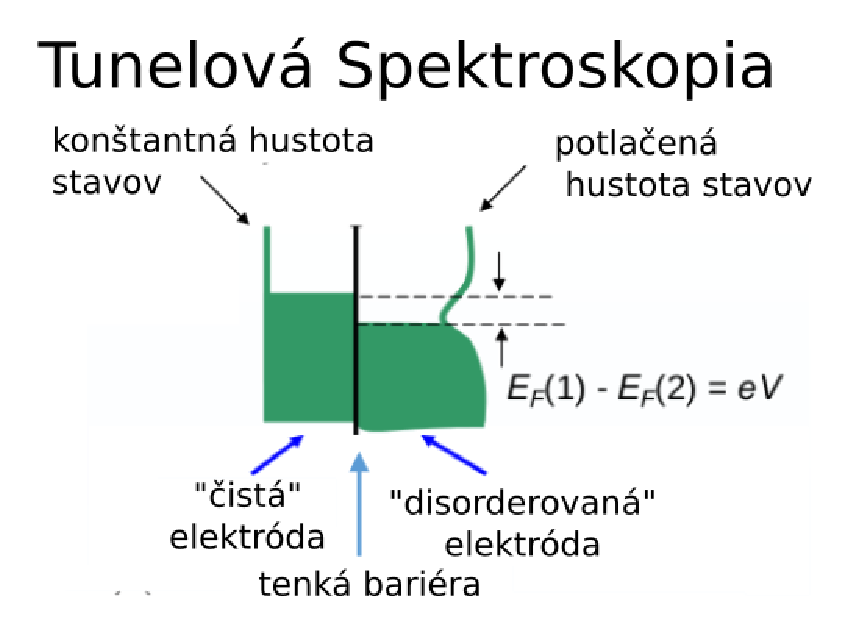
\includegraphics[scale=0.7]{grafy/DOS-sk.eps}
 \end{center}
 \caption{Meranie hustoty stavov tunelovou spektroskopiou. V experimente máme "čistý" a "disorderovaný" kov, 
 oddelené sú tenkou vrstvou izolantu, ktorý tvorí potenciálovú bariéru. Meraná veličina je diferenciálna
 vodivosť $\frac{dI(U)}{dU}=G(U)$. Vzťah medzi diferenciálnou vodivosťou a hustotou stavov je 
 $\frac{\rho(\epsilon)}{\rho_0(0)}=\frac{G(U)}{G_0(U)}$; kde $G_0$ je diferenciálna vodivosť v prípade, 
 že na oboch stranách máme "čistý" kov.}
 \label{fig:exp_dos_meranie}
\end{figure} 
Hľadanú hustotu stavov máme teraz pod integrálom. Preto je vhodné určiť difernciálnu vodivosť:
\begin{equation}
 \label{eq:exp_current_der}
  \frac{dI}{dU}=e\frac{4\pi|t^2|}{\hbar} N_l(\mu_l) N_r(\mu_r-Ue)
\end{equation} 
Deriváciu prúdu podľa napätia určíme z I-V charakteristiky. Hustotu stavov vieme vyjadriť ako funkciu merateľných veličín.
\begin{equation}
 \label{eq:exp_dos}
 N_r(\mu_r-Ue)= \frac{\frac{dI}{dU}(U)}{e\frac{4\pi|t^2|}{\hbar}}=\alpha \frac{dI}{dU}(U)
\end{equation} 
kde konštantu $\alpha$ môžme určiť fitovaním.

Pri odvodení vzťahu pre deriváciu prúdu \eqref{eq:exp_current_der} sme predpokladali, že od napätia závisí iba hustota stavov.
Vo všeobecnosti to však nieje pravda, pretože aj tunelový koeficient $t(U)$ je funkciou napätia. V našom prípade lineárne klesajúcej bariéry
tým získa meraná hustota stavov \eqref{eq:exp_dos} parabolické pozadie. 
\begin{figure}[H]
\begin{center}
 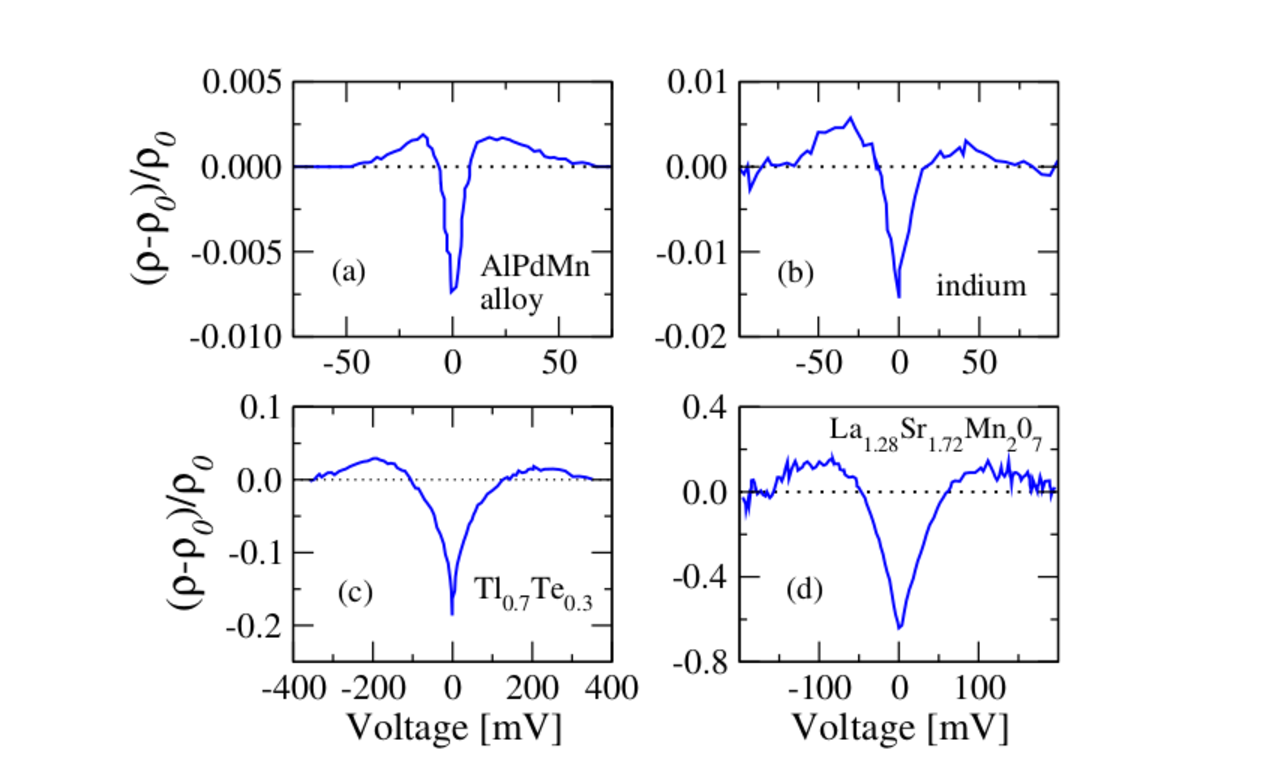
\includegraphics[scale=0.7]{grafy/B2}
 \end{center}
 \caption{Výsledky merania hustoty stavov tunelovou spektroskopiou pre rôzne kovy a zliatiny. Vo výsledných grafoch 
 môžme vidieť pokles hustoty stavov v okolí Fermiho energie}
 \label{fig:exp_results} 
\end{figure}





%%%%%%%%%%%%%%%%%%%%%%%%%%%%%%%%%%%%%%%%%%%%%%%%%%%%%%%%%%%%%%%%%%%%%%%%%%%%%%%%%%%%%%%%%%%%%%%%%%%%%%%%%%%%%%%

%%%%%%%%%%%%%%%%%%%%%%%%%%%%%%%%%%%%%%%%%%%%%%%%%%%%%%%%%%%%%%%%%%%%%%%%%%%%
%%%%%%%%%%%%%%%%%%%%%%%%%%%%%%%%%%%%%%%%%%%%%%%%%%%%%%%%%%%%%%%%%%%%%%%%%%%%
%časť diplomovka
%%%%%%%%%%%%%%%%%%%%%%%%%%%%%%%%%%%%%%%%%%%%%%%%%%%%%%%%%%%%%%%%%%%%%%%%%%%%

%\section {Experimentálne meranie hustoty stavov v disorderovanom kove}
V tejto kapitole predstavíme experimentálnu metódu merania hustoty stavov
Táto metóda využíva efekt tunelovania elektrónu cez potenciálovú bariéru.

Experimentálna sústava pozostáva z dvoch kovov odelených izolantom. Naľavo máme čistý 
kov, ktorého hustotu poznáme - {\it známy kov}. Napravo máme disorderovaný kov, ktorého 
hustotu stavov budeme merať - {\it skúmaný kov}. Izolant tvorí potenciálovú bariéru.
Na sústavu priložíme napätie  $U$ a budeme merať prúd.  

Bez priloženého napätia ($U=0$) popisuje Hamiltonián 
\begin{equation}
 \label{eq:02barrier}
 \hat{H}=\frac{\hbar^2 \laplace }{2m}+V(x) \text{,}
\end{equation} 
kde 
\begin{equation}
 \label{eq:02potential_barrier}
 V(x)=
 \begin{cases}
    V_0,& \text{pre } 0<x<b\\
    0,              & \text{inak}
\end{cases}\text{,}
\end{equation} 
kde $b$ je šírka bariéry,

Hladanie vlastných stavov Hamiltoniánu \eqref{eq:02barrier} je učebnicový problém, ktorý sa 
štandartne rieši nájdením vlnových funkcii v troch oblastiach a následným ,,zošívaním'' 
pomocou podmienky spojitosti vlnovej funkcie a jej derivácie. 

Štandartný spôsob riešenia však zlyhá po priložení napätia na experimentálnu sústavu. 
Preto predstavíme iný spôsob.

Majme teraz dve nekonečne široké bariéry z ľava:
\begin{equation}
 \label{eq:02potential_left}
 V_l(x)=
 \begin{cases}
    V_0,& \text{pre } 0<x\\
    0,              & \text{inak}
\end{cases}\text{,}
\end{equation}
a podobne sprava
 \begin{equation}
 \label{eq:02potential_right}
 V_r(x)=
 \begin{cases}
    V_0,& \text{pre } b>x\\
    0,              & \text{inak}
\end{cases}\text{.}
\end{equation}
Pre obe bariéry \eqref{eq:02potential_left} a \eqref{eq:02potential_right} vieme určiť 
vlastné stavy $\psi_{l}(x)$ a $\psi_{r}(x)$. Tieto stavy sú očividne dobrou aproximáciou 
stavov naľavo a napravo od konečnej bariéry \eqref{eq:02potential_barrier}. Nie sú to však 
vlastné stavy hamiltoniánu \eqref{eq:02barrier}, preto musíme riešiť časovú SchR 
\begin{equation}
 \label{eq:02time_schr}
 i\hbar \frac{d}{dt}\psi(x,t)=\hat{H} \psi(x,t)\text{.}
\end{equation} 
Časticu je v čase $t=0$ na ľavo od bariéry teda v stave $\psi_l(x)$, teda máme počiatočnú 
podmienku 
\begin{equation}
 \label{eq:02init_cond} 
 \psi(x,0)=\psi_l(x)\text{.}
\end{equation}
Riešenie časovej SchR \eqref{eq:02time_schr} hľadáme v tvare:
\begin{equation}
 \label{eq:02time_schr_solution}
 \psi(x,t)=c_l(t)\psi_l(x)e^{-\frac{iE_l t}{\hbar}}+\sum_{\forall r} c_r(t)\psi_l(x)e^{-\frac{iE_r t}
{\hbar}}\text{,}
\end{equation}  
kde s počiatočných podmienok \eqref{eq:02init_cond} dostávame:
\begin{equation}
 \label{eq:02time_schr_coeficients} 
c_l(0)=1 , c_r(0)=0 \text{.}
 \end{equation} 
 Pre slabo preniknuteľnú bariéru vieme koeficienty aproximovať ako:
 \begin{equation}
 \label{eq:02time_schr_coeficients_approx} 
c_l(t)\doteq1,c_l'(t)\doteq1 , c_r(t)\doteq0 \text{.}
 \end{equation} 
 
Dosadením \eqref{eq:02time_schr_solution}  do \eqref{eq:02time_schr} a použitím 
\eqref{eq:02time_schr_coeficients_approx} 
a následnými úpravami  dostávame
\begin{equation}
 \label{eq:02golden_rule}
 w_{r\to l}=\frac{2\pi}{\hbar} \bra{\psi_l}H-E_l\ket{\psi_r}\delta(E_l-E_r)\text{.}
\end{equation} 
Dostali sme vzťah podobný Fermiho zlatému pravidlu, ktorý popisuje pravdepodobnost 
prechod zo stavu $\psi_l$  do stavu $\psi_r$. 

V ďalšom zavedieme označenie
\begin{equation}
\label{eq:02t}
t_{k_l \to k_r}=\bra{\psi_l}H-E_l\ket{\psi_r}
\end{equation}

Teraz priložíme na sústavu napätie $U$, čo spôsobí zmenu dna energetického pásu na 
pravej strane bariéry $\Delta E_c$.  Potenciálová bariéra má teraz tvar lineárnej funkcie.
Obsadzovacie čísla jednotlivých elektrónových stavov budú na ľavo dané Fermi-Diracovým rozdelením:
\begin{equation}
 \label{eq:02fermidirac_left}
 f_l(k_l)=\frac{1}{e^{\frac{E_{k_l}-\mu_l}{k_bT}}+1}\text{,}
\end{equation} 

podobne pre stavy na pravo:

\begin{equation}
 \label{eq:02fermidirac_right}
 f_r(k_r)=\frac{1}{e^{\frac{E_{k_r}-\mu_r}{k_bT}}+1}\text{.}
\end{equation} 

Počet elektrónov ktoré prejdu zľava do prava, resp sprava do ľava.
\begin{equation}
\label{eq:02elctronsLTR}
\Gamma^+(\Delta E)=\sum_{k_l}{\sum_{k_r} w_{k_l \to k_r} f_l(k_l)[1-f_r(k_r)]}
\end{equation}

\begin{equation}
\label{eq:02elctronsRTL}
\Gamma^-(\Delta E)=\sum_{k_l}{\sum_{k_r} w_{k_r \to k_l} f_r(k_r)[1-f_l(k_l)]}
\end{equation}

Kde $\Delta E$ je rozdiel energii medzi stavmi naľavo a napravo, pozri obrázok. Celkový prúd je teda 
\begin{equation}
\label{eq:02current}
I={\Gamma^+(\Delta E) - \Gamma^-(\Delta E)}
\end{equation}


V roviniciach \eqref{eq:02elctronsLTR} a \eqref{eq:02elctronsRTL}  prejdeme od sumy k integrálu a dosadíme Zlaté pravidlo \eqref{eq:02golden_rule}. Nakoniec prejdeme k integrálu cez energiu, kde musíme násobiť hustotu stavov.
\begin{align*}
\Gamma^+(\Delta E)=\frac{2\pi}{\hbar}2\sum_{k_l} \sum_{k_r} {|t_{k_l \to k_r}|^2f_l(k_l)[1-f_r(k_r)]\delta(E_{l}-E_{r})}= \\
\frac{2\pi}{\hbar}2 \int_{0}^{\infty}\frac{L}{\pi} dk_{r}\int_{0}^{\infty}\frac{L}{\pi} dl_{l} {|t_{k_l \to k_r}|^2f_l(k_l)[1-f_r(k_r)]\delta(E_{l}-E_{r})} \simeq\\
 \frac{2\pi}{\hbar}2 |t|^2 \int_{E_{c,l}}^{\infty}\frac{L}{\pi}\rho_r(E_r)dE_r\int_{E_{c,r}}^{\infty}\frac{L}{\pi} N_r(E_r)dE_r {f_l(k_l)[1-f_r(k_r)]\delta(E_{l}-E_{r})} \text{,}\\
\end{align*}
kde sme v poslednom riadku zanedbali závislosť transmisného koeficientu $t(k_l,k_r)$ . Podobným spôsobom vieme upraviť aj vzťah \eqref{eq:02elctronsRTL}.
Takto upravené vzťahy dosadíme do rovnice pre celkový prúd prechádzajúci sústavou \eqref{eq:02current} a dostaneme 
\begin{equation}
\label{eq:02current2}
I=e\frac{4\pi|t|^2}{\hbar}\int_{E_{cl}}^\infty dE_l\rho_l(E_l)\rho_r(E_l)(f_l(E_l)-f_r(E_l)) \text{,}
\end{equation}
kde sme navyše využili $\delta$-funkciu a zbavili sa integrovania cez $E_r$. 


V limite nízkych teplôt $T \simeq 0$ Fermi-Diracove funkcie prejdú na $\Theta$-funkcie. Preto dostávame
\begin{align}
I=e\frac{4\pi|t|^2}{\hbar}[\int_{E_{cl}}^{\mu_l}dE_l-\int_{E_{cl}}^{\mu_r}dE_l\rho_r(E_l)\rho_l(E_l)]\text{,}
\end{align}
Chemické potenciály na ľavej a pravej strane bariéry $\mu_r$ a $\mu_l$ sa líšia o $-Ue$ teda integrál napíšeme ako
\begin{align}
\label{eq:02current3}
I = e \frac{4\pi|t|^2}{\hbar}\int_{\mu_r}^{\mu_r-Ue}dE_l\rho_r(E_l)\rho_l(E_l)\text{.}
\end{align}
 Na ľavej strane bariéry je známy kov bez disorderu. Jeho hustota stavov sa v okolí Fermiho energie dá aproximovať konštantou. Fermiho energia (a teda aj chemický potenciál naľavo $\mu_l$ i napravo $\mu_r$ )je rádovo $E_F\sim\SI{10}{\eV}$ a rozdiel enregí je rádovo $eU\sim \SI{100}{\milli\eV}$, teda na celom intervale integrálu v
\eqref{eq:02current3} možno nahradiť hustotu stavov $\rho_l(E_l)$ konštantou $\rho_1(\mu_l)$, čiže hustotou stavov na Fermiho hladine. Konštantu vyjmeme pred integrál a dostaneme
\begin{align}
I = e \frac{4\pi|t|^2}{\hbar}\rho_l(\mu_l)\int_{\mu_r}^{\mu_r-Ue}dE_l\rho_r(E_l)\text{,}
\end{align}
teda pre diferenciálnu vodivosť dostaneme
\begin{align}
\label{eq:02diff}
\frac{d I}{d U}=e\frac{4\pi|t|^2}{\hbar}\rho_l(\mu_l)\rho_r(\mu_r-Ue)
\end{align}
Diferenciálnu vodivosť vieme experimentálne merať, a to určením voltampérovej charakteristiky. Preto z \eqref{eq:02diff} vyjaderíme jedinú neznámu veličinu, hustotu stavov skúmaného kovu napravo. Dostaneme priamu úmernosť medzi difernciálnou vodivosťou a hustotou stacvov 
\begin{align}
\rho_r(\mu_r-Ue)=\alpha \frac{d I}{d U} \text{,}
\end{align}
kde $\alpha=\frac{\hbar}{4\pi|t|^2e}$ je konštanta úmernosti. 

Hustotu stavov meriame určením voltampérovej charakteristiky sústavy {\it známy} kov - bariéra (izolant) - {\it skúmaný} kov, ktorá je po prenásobení konštantou $\alpha$ hustota stavov. {\it Známy} kov musí byť čistý (bez disorderu) aby sme v okolí Fermiho energie mohli použiť parabolický disperzný zákon a týmpádom aproximáciu $\rho_l(E_l)\approx\rho_l(\mu_l)$. 

Pri meraní vložíme najskôr na obe strany čistý kov, a určíme jeho diferenciálnu vodivosť, ktorú označíme  $G_0(U)$. Potom meriame diferenciálnu vodivosť sústavy s disorderovaným kovom napravo $G(U)=\frac{dI(U)}{dU}$. 

Pre hustotu stavov skúmaného kovu dostaneme:
\begin{align}
\frac{\rho_r(E)}{\rho_l(E_F)} = \frac{G(U)}{G_0(U)}
\end{align}

Kde $\rho_l(E_F)$ je daná parabolickým disperzným zákonom.
\begin{figure}[H]
\centering
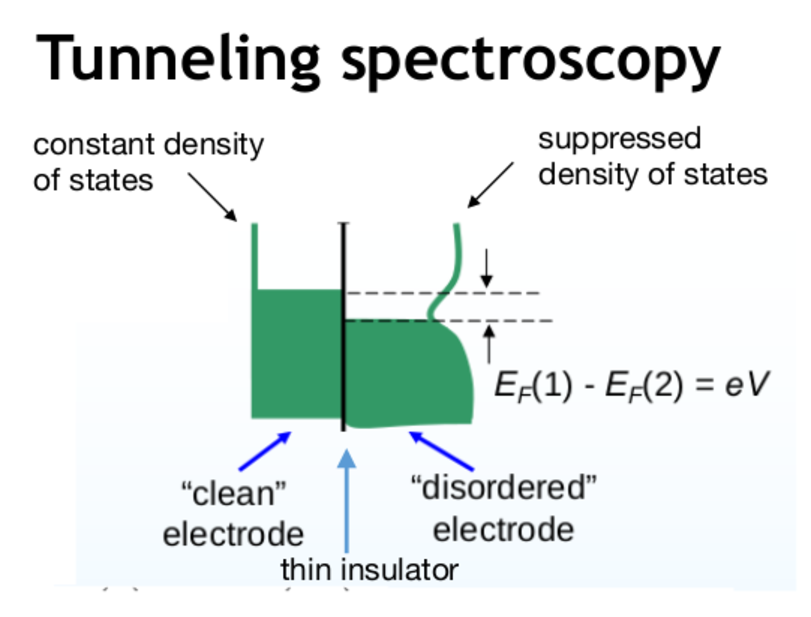
\includegraphics[scale=1]{grafy/DOS-cropped}
\caption{Meranie hustoty stavov tunelovou spektroskopiou. V experimente máme "čistý" a "disorderovaný" kov oddelené tenkou vrstvou izolantu. Meraná veličina je difernciálna vodivosť $\frac{d I}{d U}$}. 
\end{figure}
\begin{figure}[H]
\centering
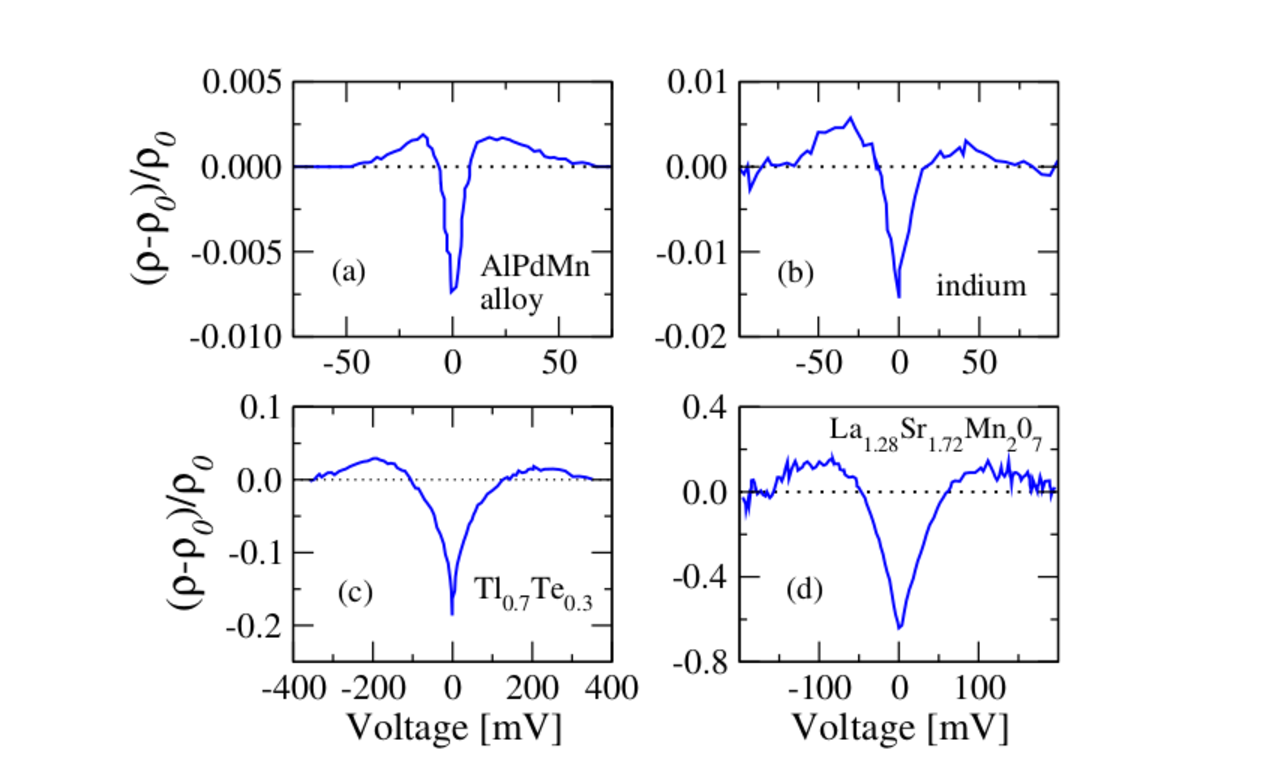
\includegraphics[scale=1]{grafy/B2}
\caption{Výsledky merania hustoty stavov tunelovou spektroskopiou pre rôzne zliatiny. Vo výsledných grafoch môžme vidieť pokles hustoty stavov v okolí Fermiho Energie, podľa predpovedí Altschulera-Aronova. Zároveň vidíme  nárast hustoty stavov v oblasti ďalej od $E_F$.}
\end{figure}